%\chapter{Simulador Gazebo}

%Este capítulo explicita três elementos do simulador Gazebo utilizados na criação do ambiente de desenvolvimento ProVANT: 
%
%\begin{itemize}
%	\item[\textbf{Modelo}] conjunto de arquivos com informações relativas à estrutura física do vant: características inerciais, visuais e de colisão.
%	\item[\textbf{Cenário}] arquivo de descrição de configurações da simulação, tal como passo de simulação, tipo de motor de simulação, elementos visuais (exemplo: ventos, céu, e cor do piso) e quantidade/pose inicial de modelos.
%	\item[\textbf{Plugin}] código fonte de criação de elementos sensoriais e de atuação do modelos.
%\end{itemize}

\chapter{Modelos}

\section{Organização e estrutura}


\begin{tiny}
	\begin{figure}[H]
		\begin{forest}
			for tree={font=\sffamily, grow'=0,
				folder indent=.9em, folder icons,
				edge=densely dotted}
			[vant\_x
			[config
			[config.xml, is file]  
			]
			[meshes
			[$\star$.stl,is file]
			]  
			[robot
			[model.sdf, is file]
			]
			[imagem.gif, is file]
			[model.config, is file]
			]
		\end{forest}
		\caption{Árvore ilustrativa para um diretório que descreve um VANT de versão x \emph{vant\_x}.}
		\label{fig:arvore_vantx}
	\end{figure}
\end{tiny}


Os arquivos associados aos modelos de VANTs, utilizados no ambiente de simulação ProVANT, estão localizados na pasta referênte ao caminho:

\begin{bashcode}
$HOME/catkin_ws/src/ProVANT-Simulator/source/Database/models/real
\end{bashcode}


Cada modelo no ambiente de simulação ProVant possui um diretório com o seu respectivo nome. Nesse diretório estão arquivos que descrevem os modelos dinâmicos, visuais, de colisão, sensoriais e da lei de controle utilizada. Portanto, caso seja necessário adicionar um novo modelo, ou editar um existente, o mesmo deve possuir arquivos de configuração/descrição do VANT organizados conforme ilustrado na Figura \ref{fig:arvore_vantx}. Os diretórios e arquivos necessários são:
 
\begin{itemize}
\item\emph{config}:  a pasta \emph{config} possui um único arquivo nomeado \emph{config.xml}. Este arquivo em \emph{XML} escreve configurações do Controlador, tais como período de amostragem e estratégia de controle a ser utilizada, e será explicitado no capítulo referente a descrição do elemento Controlador.
\item \emph{meshes}: a pasta contêm os arquivos de extensão \emph{.stl} que são obtidos no processo de importação do modelo em CAD do VANT pelo \emph{Solidworks}.
\item \emph{robot}: a pasta contêm um arquivo \emph{SDF} que descreve o VANT para o simulador.
\item \emph{imagem.gif}: corresponde à imagem do vant a ser utilizada na interface gráfica.
\item \emph{model.config}: arquivo \emph{XML} com informações sobre o modelo, o nome do desenvolvedor e as licenças de uso.
\end{itemize}



\section{Arquivo ''model.sdf''}


Antes de apresentar a configuração básica de um arquivo SDF, é necessário primeiro introduzir alguns conceitos. Um modelo corresponde a um sistema mecânico, que pode ser formado por um ou múltiplos corpos rígidos\footnote{Ao assumir um corpo como rígido são desprezando efeitos de elasticidade e deformações}. Assim como em um manipulador, no simulador os corpos são denominados elos. Elos filhos são conectados a elos pai através de juntas. Elos filhos são corpos rígidos que possuem movimento restringido pela conexão ("junta") com corpos denominados elos pai. Os elos possuem propriedades inerciais, visuais e de colisão. Já as juntas, impõem a restrição do movimento relativo entre dois elos, com propriedades como o tipo de junta (Prismática, rotativa, etc.), limites de movimento (Posição e velocidade), existência de atrito, etc. A Figura \ref{geral} ilustra um exemplo de arquivo SDF, onde:\small
\begin{itemize}
\setlength{\itemsep}{1pt}
\setlength{\parskip}{0pt}
\setlength{\parsep}{0pt}
\item[-] \textcolor{blue}{<link></link>}: especifica a existência de um elo, com o seu nome;
\item[-] \textcolor{blue}{<joint></joint>}: especifica a existência de uma junta, com o seu nome.  
\end{itemize}\normalsize

\begin{figure}[H]
\begin{minted}{xml}
<?xml version="1.0" encoding="UTF-8"?>
<sdf version="1.4">
	<model name="modelo">
		<link name="corpo">
		...
		</link>
		<link name="servo">
		...
		</link>
		<joint name="corpo_servo">
		...
		</joint>
	</model>
</sdf>
\end{minted}
\vspace{-1cm}
\caption{Descrição de um elo no arquivo ''modelo.sdf''}
\label{geral}
\end{figure}


Cada elo do modelo possui três tipos de descrições para o simulador: cinemática, visual e de colisão.  A estrutura de configuração de um elo em um arquivo SDF possui o formato ilustrado na Figura \ref{elo}, onde:
\small
\begin{itemize}
\setlength{\itemsep}{1pt}
\setlength{\parskip}{0pt}
\setlength{\parsep}{0pt}
\item[-] \textcolor{blue}{<pose></pose>}: define a pose do elo;
\item[-] \textcolor{blue}{<inertial></inertial>}: especifica as propriedades inerciais do elo;
\item[-] \textcolor{blue}{<collision></collision>}: especifica o modelo de colisão do elo. Os modelos de colisão dos VANTs usados no ambiente de simulação são obtidos de arquivos CAD;
\item[-] \textcolor{blue}{<visual></visual>}: especifica características visuais, como cor e formato. Os modelos visuais dos VANTs usados no ambiente de simulação são obtidos de arquivos CAD, exceto a cor, que é especificada separadamente.
\end{itemize}\normalsize

\begin{figure}[ht!]
\begin{minted}{xml}
<link name="servodir">
	<pose>0.02E-3 -277.61E-3 56.21E-3 -0.0872665 0 0</pose>
	<inertial> 
	...
	</inertial>
	<collision name="servodircollision"> <!--opcional-->
	...
	</collision>
	<visual name="servodirvisual"> <!--opcional-->
	...
	</visual>
</link>
\end{minted}
\vspace{-1cm}
\caption{Descrição da de um elo no ''modelo.sdf''}
\label{elo}
\end{figure}

\noindent \textbf{Parâmetros de inércia do elo}: O usuário deve informar os parâmetros de inércia de cada elo na \textit{tag} ''inertial''. As informações obrigatórias são a massa, posição relativa do centro de massa e o tensor de inércia. Na Figura \ref{inertial} é ilustrado um exemplo de configuração dos parâmetros de inércia de um elo em formato SDF, onde:
\small
\begin{itemize}
\setlength{\itemsep}{1pt}
\setlength{\parskip}{0pt}
\setlength{\parsep}{0pt}
\item[-] \textcolor{blue}{<mass></mass>}: define a massa do elo;
\item[-] \textcolor{blue}{<pose></pose>}: especifica a posição do centro de massa do elo em relação a seu sistema de coordenadas principal;
\item[-] \textcolor{blue}{<inertia></inertia>}: especifica o tensor de inércia do elo;
\end{itemize}\normalsize

\begin{figure}[H]
\begin{minted}{xml}
<inertial>
	<mass>0.0809439719362664</mass>
	<pose>
	-3.60859273452335E-10 -0.000226380714807978 0.0594780519701684 0 0 0
	</pose>
	<inertia>
		<ixx>3.88267747087835E-06</ixx>
		<ixy>6.03219085082653E-06</ixy>
		<ixz>-2.78471406661236E-12</ixz>
		<iyy>0.000104858690365283</iyy>
		<iyz>7.0486590219062E-07</iyz>
		<izz>8.31755564684115E-05</izz>		
	</inertia>
</inertial>
\end{minted}
\vspace{-0.8cm}
\caption{Descrição de características inerciais no arquivo ''modelo.sdf''}
\label{inertial}
\end{figure}


\noindent \textbf{Propriedades de colisão do elo}: Para que efeitos de colisão sejam aplicados ao elo, o usuário deve descrever o formato do elo no arquivo ''model.sdf''. Existem diversas formas de descrição, porém este manual apresenta apenas o método utilizado nos modelos de VANTs do ambiente de simulação ProVANT, que consiste na importação de arquivos criados através de ferramentas CAD, como o SolidWorks. A Figura \ref{colision} mostra um exemplo de descrição dos parâmetros visuais de um elo a partir de um arquivo STL, onde:
\small
\begin{itemize}
\setlength{\itemsep}{1pt}
\setlength{\parskip}{0pt}
\setlength{\parsep}{0pt}
\item[-] \textcolor{blue}{<pose></pose>}: especifica a pose do modelo colisão em relação ao centro de coordenadas do elo;
\item[-] \textcolor{blue}{<uri></uri>}: caminho do arquivo mesh, a partir do diretório do modelo, obtido via exportação no SolidWorks; 
\end{itemize} \normalsize

\begin{figure}[ht!]
\begin{minted}{xml}
<collision name="servodircollision">
	<pose>0 0 0 0 0 0</pose>
	<geometry>
		<mesh>
			<uri>model://vant_2comcarga/meshes/servodir.STL</uri>
		</mesh>
	</geometry>
</collision>
\end{minted}
\vspace{-0.8cm}
\caption{Descrição de características de colisão no arquivo ''model.sdf''}
\label{colision}
\end{figure}

\noindent \textbf{Propriedades visuais do elo}: Para que o elo seja visualizado durante a simulação, o usuário deve descrever os parâmetros visuais do elo no arquivo ''model.sdf''. Assim como no caso anterior, existem diversas formas de descrição, porém este manual ilustra apenas o método utilizado nos modelos de VANTs do ambiente de simulação, que consiste na importação de arquivos criados através de ferramentas CAD. A Figura \ref{visual} mostra um exemplo de descrição dos parâmetros visuais de um elo a partir de um arquivo STL, 	
onde: \small
\begin{itemize}
\setlength{\itemsep}{1pt}
\setlength{\parskip}{0pt}
\setlength{\parsep}{0pt}
\item[-] \textcolor{blue}{<pose></pose>}: especifica a pose que o modelo visual do elo será definido em relação ao sistema de coordenadas do elo;
\item[-] \textcolor{blue}{<uri></uri>}: caminho do arquivo mesh, a partir do diretório do modelo, obtido via exportação no SolidWorks;
\item[-] \textcolor{blue}{<ambient></ambient>}: definição de cor ambiente;
\item[-] \textcolor{blue}{<diffuse></diffuse>}: definição de cor difusa;
\item[-] \textcolor{blue}{<specular></specular>}: definição de cor especular;
\item[-] \textcolor{blue}{<emissive></emissive>}: definição de cor emissiva.
\end{itemize} \normalsize

\begin{figure}[ht!]
\begin{minted}{xml}
<visual name="servodirvisual">
	<pose>0 0 0 0 0 0</pose>
	<geometry>
		<mesh>
			<uri>model://vant_2comcarga/meshes/servodir.STL</uri>
		</mesh>
	</geometry>
	<material>
		<ambient>0 0 0 0</ambient>
		<diffuse>1 1 1 1</diffuse>
		<specular>0.1 0.1 0.1 1</specular>
		<emissive>0 0 0 0</emissive>
	</material>
</visual>
\end{minted}
\vspace{-0.8cm}
\caption{Descrição de características visuais no arquivo ''model.sdf''}
\label{visual}
\end{figure}

\subsubsection{Descrição de junta} 

Há 7 tipos de juntas no simulador: 

\begin{itemize}
\item \textbf{revolute}: junta rotativa; 
\item \textbf{gearbox}: junta rotativa com presença de engrenagens para transmissão de movimento angular entre elos com diferentes relações de torque e velocidade; 
\item \textbf{revolute2}: junta composta por duas juntas rotativas em série; 
\item \textbf{prismatic}: junta prismática; (\textbf{universal}), junta com comportamento de uma bola articulada; 
\item \textbf{piston}: junta com comportamento da combinação de uma junta rotativa e uma junta prismática.
\end{itemize}

Um exemplo de estrutura de configuração de uma junta é mostrado na Figura \ref{joint}, onde:
\begin{itemize}
\setlength{\itemsep}{1pt}
\setlength{\parskip}{0pt}
\setlength{\parsep}{0pt}
\item[-] \textcolor{blue}{<pose></pose>}: descreve a pose relativa em que o elo filho está em relação ao elo pai.
\item[-] \textcolor{blue}{<parent></parent>}: nome do elo pai.
\item[-] \textcolor{blue}{<child></child>}: nome do elo filho.
\item[-] \textcolor{blue}{<axis></axis>}: vetor unitário que corresponde ao eixo de rotação da junta. (expressado no sistema de coordenadas do modelo, se estiver utilizando a versão 1.4 do formato SDF; e expressado no sistema de coordenadas do elo filho, se estiver utilizando a versão 1.6 do formato SDF).
\item[-] \textcolor{blue}{<lower></lower>}: limite inferior de posição da junta (em rad, caso seja do tipo rotativa, e metros, caso seja prismática).
\item[-] \textcolor{blue}{<upper></upper>}: limite superior de posição da junta (em rad, caso seja do tipo rotativa, e metros, caso seja prismática).
\item[-] \textcolor{blue}{<velocity></velocity>}: limite de velocidade da junta (em rad/s, caso seja do tipo rotativa, e m/s, caso seja prismática).
\item[-] \textcolor{blue}{<effort></effort>}: limite de esforço da junta (em N.m, caso seja do tipo rotativa, e N, caso seja prismática).
\item[-] \textcolor{blue}{<damping></damping>}: coeficiente de atrito viscoso.
\item[-] \textcolor{blue}{<friction></friction>}: coeficiente de atrito estático.
\end{itemize}

\begin{figure}[ht!]
\begin{minted}{xml}
<joint name="aR" type="revolute">
	<pose>0 0 0 0 0 0</pose>
	<parent>corpo</parent>
	<child>servodir</child>
	<axis>
		<xyz>0 0.9962 -0.0872</xyz>
		<limit>
			<lower>-1.5</lower>
			<upper>1.5</upper>
			<effort>2</effort>
			<velocity>0.5</velocity>
		</limit>
		<dynamics>
			<damping>0</damping>
			<friction>0</friction>
		</dynamics>
	</axis>
</joint>
\end{minted}
\vspace{-0.8cm}
\caption{Descrição de juntas no arquivo ''model.sdf''}
\label{joint}
\end{figure}

\section{Arquivo ''model.config''}

No arquivo ''model.config'' o gazebo identifica onde está o arquivo com os dados estruturais do modelo, além de informações associadas à autoria, versão e descrição do modelo. A Figura \ref{model.config} ilustra um exemplo desse arquivo. As \textit{tags} utilizadas no arquivo ''model.config'' são:
\small
\begin{itemize}
\setlength{\itemsep}{1pt}
\setlength{\parskip}{0pt}
\setlength{\parsep}{0pt}
\item[-] \textcolor{blue}{<name></name>}: especifica o nome do modelo;
\item[-] \textcolor{blue}{<version></version>}: especifica a versão;
\item[-] \textcolor{blue}{<sdf></sdf>}: especifica o arquivo com a descrição do modelo dinâmico, de colisão e visual de modelo para o simulador Gazebo;
\item[-] \textcolor{blue}{<author><name></name></author>}\textcolor{blue}: especifica o nome do autor do modelo;
\item[-] \textcolor{blue}{<author><email></email></author>}: especifica o email para contato com o autor;
\item[-] \textcolor{blue}{<description></description>}: descreve brevemente o modelo.
\end{itemize}\normalsize

\begin{figure}[ht!]
\begin{minted}{xml}
<?xml version="1.0"?>
<model>
<name>vant</name>
<version>1.0</version>
<sdf version='1.5'>robot/model.sdf</sdf>
	<author>
	<name>provant</name>
	<email>provant@ufmg.br</email>
	</author>
		<description>
			The UAV version 3.0 of the provant project 
		</description>
	</model>
</sdf>
\end{minted}
\vspace{-0.8cm}
\caption{Exemplo de conteúdo existente no arquivo ''model.config''}
\label{model.config}
\end{figure}


\section{Arquivos ''meshes''}

''Mesh'' (do inglês, significa malha) é a representação de objetos virtuais/computacionais em várias áreas da tecnologia, sobretudo na resoluções de problemas de engenharia e é compostas por vértices, arestas e triângulos.

O simulador Gazebo consegue importar dois tipos de arquivos para representação de área e superfícies: arquivos STL e DAE, estes oriundos de softwares CAD. No ambiente de simulação ProVANT, cada modelo vant é formado por vários elos e cada elo terá respectivas representações visuais e de colisão. Por motivos de organização, definiu-se que e o diretório ''Meshes'' será o local para armazenamento de tais arquivos.

A seguir será demonstrado um passo a passo de como obter o modelo com seus respectivos arquivos de descrição visual e de colisão.    

\section{Obtenção de modelos a partir do SolidWorks}

Está subseção descreve o conjunto de passos necessários para a exportação de um projeto mecânico para o formato necessário para uso no simulador Gazebo. Atente-se à necessidade de realizar ajustes no desenho CAD para o processo de exportação tenha sucesso. 

\subsection{Ajustes no Desenho CAD }

Para poder exportar o modelo para o formato necessário para uso no simulador Gazebo é necessário realizar o \textit{download} e instalação do plugin ''Sw\_Urdf\_Exporter''. O plugin pode ser encontrado em \url{http://wiki.ros.org/sw_urdf_exporter}. 

Além de \textit{download} e instalação do plugin, é necessário garantir que não exista nenhuma peça com o valor da massa substituída manualmente. Isso gera inconsistências entre o modelo em CAD e o modelo exportado. Uma maneira solucionar este problema, é criar um material personalizado, com uma densidade que corresponda a massa desejada, tal valor é obtido através da relação entre massa e volume.

Outro ajuste importante é a definição de quantos elos deve ter o modelo. Neste manual, exemplifica-se o processo de exportação para o modelo VANT-3.0, ilustrado na Figura \ref{vant.jpg}.

O VANT 3.0, ao todo possui sete corpos:


\begin{description}
\item [main\_body] é o corpo referência do VANT-3.0, composto pelo Corpo, suporte dos motores e parte fixa da empenagem;
\item [motorR] é o grupo propulsor da direita com exceção da hélice; 
\item [motorL] é o grupo propulsor da esquerda com exceção da hélice; 
\item [propeller\_R] é a hélice da direita;
\item [propeller\_L] é a hélice da esquerda;
\item [elevator] é a parte móvel da empenagem horizontal;
\item [rudder] é a parte móvel da empenagem vertical.
\end{description}

É necessário criar um eixo de coordenadas no centro de massa de cada um dos corpos, para que possam ser referenciados no momento da exportação. No caso do VANT-3.0 são criados eixos de coordenadas sobre o eixo de rotação dos servos. Outro eixo além dos citados é a referência do main\_body, localizado onde, teoricamente, pode-se encotrar a IMU. É importante a criação de eixos, que determinam como os corpos se movimentam, já que só temos movimentos de revolução. No VANT-3.0 existem eixos criados no centro de rotação das hélices e nos servos.E também no profundor e no leme.

\subsection{Processo de Exportação}

O processo de exportação de um arquivo ''.sdlprt'' para ''.urdf'' é simples e intuitivo. O recurso se encontra em File->Export as URDF, o endereço pode mudar entre versões do SolidWorks®, no caso foi usada a de 2014.

\begin{figure}[!htb]% aqui começa o ambiente figura
\centering % este comando é para centralizar a figura
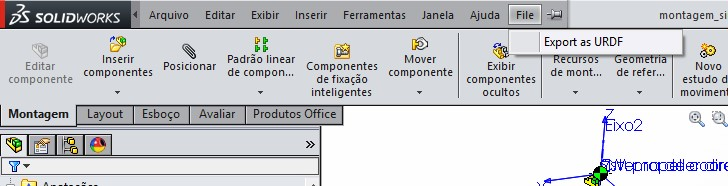
\includegraphics[scale=0.75]{Imagens/ExportasURDF.jpg} % aqui é onde chamamos a figura o que está entre [] são opções de formatação da figura e o que está entre {} é o nome da figura
\caption{Tela onde se inicia o processo} % esta é a legenda da figura
\end{figure} % aqui acaba o ambiente figura.


No canto direito da tela abrirá uma tela para inserir os parâmetros. Os primeiros parâmetros a inserir são sobre o link principal que serve de referência para o modelo, no caso do VANT-3.0 o main\_body. Os itens a serem detalhados estão listados abaixo:

\begin{description}
\item [Link Name] é o nome dado ao link principal do modelo a ser exportado;
\item [Global Origin Coordinate System] é o eixo de coordenadas que será a referência para esse link e para todo o modelo; 
\item [Link Components] local onde se define quais componentes do desenho CAD farão parte do link pai; 
\item [Number of child links] é onde se determina quantos links serão ligados ao link em questão;
\end{description}

\begin{figure}[!htb]% aqui começa o ambiente figura
\centering % este comando é para centralizar a figura
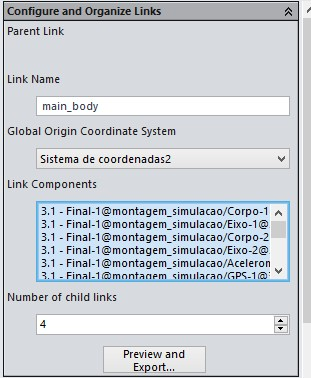
\includegraphics[scale=1]{Imagens/main_body.jpg} % aqui é onde chamamos a figura o que está entre [] são opções de formatação da figura e o que está entre {} é o nome da figura
\caption{Tela para configuração do link principal} % esta é a legenda da figura
\end{figure} % aqui acaba o ambiente figura.

Após a definição do link principal, deve-se selecionar um link filho para editar. A seleção é feita no canto inferior esquerdo, clicando-se em Emptyl\_link, como mostrado na figura abaixo.

\begin{figure}[!htb]% aqui começa o ambiente figura
\centering % este comando é para centralizar a figura
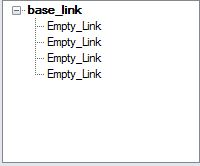
\includegraphics[scale=1]{Imagens/ArvoreVazia.JPG} % aqui é onde chamamos a figura o que está entre [] são opções de formatação da figura e o que está entre {} é o nome da figura
\caption{Tela para se iniciar a configuração de um link filho} % esta é a legenda da figura
\end{figure} % aqui acaba o ambiente figura.

Em seguida deve se editar cada link filho do modelo. Como os links filhos se movimentam, algumas informações adicionais têm que ser inseridas:

\begin{description}
\item [Link Name] é o nome dado ao link do modelo a ser exportado;
\item [Joint Name] é o nome dado a junta do modelo a ser exportado;
\item [Reference Coordinate System] é  o eixo de coordenadas que será a referência para esse link; 
\item [Reference Axis] é o eixo de referência para o movimento da junta;
\item [Joint Type] é o tipo da junta, definido pela maneira como a qual se movimenta. Pode ser por revolução, contínua, prismática ou fixa;
\item [Link Components] local onde se define quais componentes do desenho CAD farão parte do link especificado; 
\item [Number of child links] é onde se determina quantos links serão ligados ao ao link em questão;
\end{description}

\begin{figure}[!htb]% aqui começa o ambiente figura
\centering % este comando é para centralizar a figura
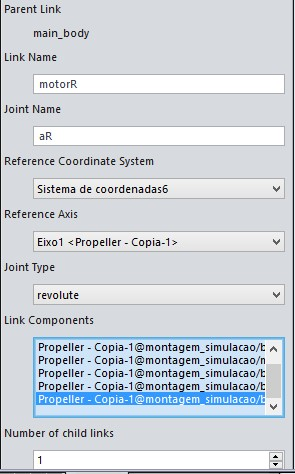
\includegraphics[scale=01]{Imagens/motorR.jpg} % aqui é onde chamamos a figura o que está entre [] são opções de formatação da figura e o que está entre {} é o nome da figura
\caption{Tela para configuração de links filhos} % esta é a legenda da figura
\end{figure} % aqui acaba o ambiente figura.

Para o VANT-3.0 foram usadas as configurações encontradas nas Tabelas \ref{tab:mainbody}, \ref{tab:servodireito}, \ref{tab:helicedireita}, \ref{tab:servoesquerdo}, \ref{tab:hélice esquerda}, \ref{tab:empenagemhorizontal} e \ref{tab:empenagemvertical}.


% Table generated by Excel2LaTeX from sheet 'Sheet1'
\begin{table}[htbp]
\centering
\begin{tabular}{|l|cccc|}
\hline
Link Name & \multicolumn{4}{c|}{ main\textbackslash{}\_body} \\
\hline
Global Origin Coordinate System  & \multicolumn{4}{c|}{Sistemas de coordenadas2} \\
\hline
\multicolumn{1}{|p{14.715em}|}{Link Components } & \multicolumn{4}{p{18.36em}|}{Todas as peças da montagem 3.1 - Final, com exceção do profundor e do leme} \\
\hline
Number of child links & \multicolumn{4}{c|}{4} \\
\hline
\end{tabular}%
\caption{Elo correspondente ao corpo principal}
\label{tab:mainbody}%
\end{table}%

% Table generated by Excel2LaTeX from sheet 'Sheet1'
\begin{table}[htbp]
\centering
\begin{tabular}{|l|c|c|c|c|}
\hline
Link Name & \multicolumn{4}{c|}{ motorR} \\
\hline
Joint Name & \multicolumn{4}{c|}{aR} \\
\hline
Reference Coordinate System  & \multicolumn{4}{c|}{Sistema de coordenadas6} \\
\hline
Reference Axis  & \multicolumn{4}{c|}{Eixo1<Propeller - Copia-1>} \\
\hline
Joint Type  & \multicolumn{4}{c|}{revolute} \\
\hline
Link Components   & \multicolumn{4}{c|}{Grupo propulsor da direita sem a hélice} \\
\hline
Number of child links  & \multicolumn{4}{c|}{1} \\
\hline
\end{tabular}%
\caption{Elo correspondente ao servo motor direito}
\label{tab:servodireito}%
\end{table}%

% Table generated by Excel2LaTeX from sheet 'Sheet1'
\begin{table}[htbp]
\centering
\begin{tabular}{|l|c|c|c|c|}
\hline
Link Name  & \multicolumn{4}{c|}{propeller\textbackslash{}\_R} \\
\hline
Joint Name  & \multicolumn{4}{c|}{thurst} \\
\hline
Reference Coordinate System   & \multicolumn{4}{c|}{Sistema de coordenadas6} \\
\hline
Reference Axis  & \multicolumn{4}{c|}{Eixo2<Propeller - Copia-1>} \\
\hline
Joint Type  & \multicolumn{4}{c|}{continuos} \\
\hline
Link Components   & \multicolumn{4}{c|}{Hélice da direita} \\
\hline
Number of child links  & \multicolumn{4}{c|}{0} \\
\hline
\end{tabular}%
\caption{Elo correspondente à helice direita}
\label{tab:helicedireita}%
\end{table}%

% Table generated by Excel2LaTeX from sheet 'Sheet1'
\begin{table}[htbp]
\centering
\begin{tabular}{|l|c|c|c|c|}
\hline
Link Name  & \multicolumn{4}{c|}{motorL} \\
\hline
Joint Name  & \multicolumn{4}{c|}{aL} \\
\hline
Reference Coordinate System   & \multicolumn{4}{c|}{Sistema de coordenadas4} \\
\hline
Reference Axis  & \multicolumn{4}{c|}{Eixo1<Propeller - Copia-2>} \\
\hline
Joint Type  & \multicolumn{4}{c|}{revolute} \\
\hline
Link Components   & \multicolumn{4}{c|}{Grupo propulsor da esquerda sem a hélice} \\
\hline
Number of child links & \multicolumn{4}{c|}{1} \\
\hline
\end{tabular}%
\caption{Elo correspondente ao servo esquerdo}
\label{tab:servoesquerdo}%
\end{table}%

% Table generated by Excel2LaTeX from sheet 'Sheet1'
\begin{table}[htbp]
\centering
\begin{tabular}{|l|c|c|c|c|}
\hline
Link Name  & \multicolumn{4}{c|}{popeller\textbackslash{}\_L} \\
\hline
Joint Name  & \multicolumn{4}{c|}{thurst} \\
\hline
Reference Coordinate System   & \multicolumn{4}{c|}{Sistema de coordenadas4} \\
\hline
Reference Axis  & \multicolumn{4}{c|}{Eixo2<Propeller - Copia-2>} \\
\hline
Joint Type  & \multicolumn{4}{c|}{continuos} \\
\hline
Link Components   & \multicolumn{4}{c|}{Hélice da esquerda} \\
\hline
Number of child links  & \multicolumn{4}{c|}{0} \\
\hline
\end{tabular}%
\caption{Elo correspondente à hélice esquerda}
\label{tab:hélice esquerda}%
\end{table}%

% Table generated by Excel2LaTeX from sheet 'Sheet1'
\begin{table}[htbp]
\centering
\begin{tabular}{|l|c|c|c|c|}
\hline
Link Name  & \multicolumn{4}{c|}{elevator} \\
\hline
Joint Name  & \multicolumn{4}{c|}{elev} \\
\hline
Reference Coordinate System   & \multicolumn{4}{c|}{Sistema de coordenadas9} \\
\hline
Reference Axis  & \multicolumn{4}{c|}{Eixo1<3.1 - Final/Montagem1-1>} \\
\hline
Joint Type  & \multicolumn{4}{c|}{revolute} \\
\hline
Link Components   & \multicolumn{4}{c|}{Profundor} \\
\hline
Number of child links  & \multicolumn{4}{c|}{0} \\
\hline
\end{tabular}%
\caption{Elo correpondente à empenagem horizontal}
\label{tab:empenagemhorizontal}%
\end{table}%

% Table generated by Excel2LaTeX from sheet 'Sheet1'
\begin{table}[htbp]
\centering
\begin{tabular}{|l|c|c|c|c|}
\hline
Joint Name  & \multicolumn{4}{c|}{rud} \\
\hline
Reference Coordinate System   & \multicolumn{4}{c|}{Sistema de coordenadas10} \\
\hline
Reference Axis  & \multicolumn{4}{c|}{Eixo2<3.1 - Final/Montagem1-1>} \\
\hline
Joint Type  & \multicolumn{4}{c|}{revolute} \\
\hline
Link Components   & \multicolumn{4}{c|}{Leme} \\
\hline
Number of child links  & \multicolumn{4}{c|}{0} \\
\hline
\end{tabular}%
\caption{Elo correspondente à empenagem vertical}
\label{tab:empenagemvertical}%
\end{table}%



\begin{figure}[!htb]% aqui começa o ambiente figura
\centering % este comando é para centralizar a figura
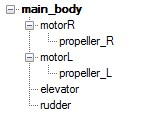
\includegraphics[scale=1.3]{Imagens/ArvoreCheia.jpg} % aqui é onde chamamos a figura o que está entre [] são opções de formatação da figura e o que está entre {} é o nome da figura
\caption{Estruturação dos links no VANT-3.0} % esta é a legenda da figura
\end{figure} % aqui acaba o ambiente figura.


Após a edição dos parâmetros deve-se clicar em 'Preview and Export...' para começar a conversão. Uma tela irá aparecer com os dados das juntas. É importante conferir os valores para assegurar um bom modelo exportado, caso em alguma junta todos os campos aparecerem em branco de ser realizada uma nova exportação. Após a verificação deve-se clicar em 'next' e realizar as mesmas conferência para os links. Não é recomendável alterar nenhum dado nessa etapa, podendo ocasionar em um modelo que não representa a realidade. Em seguida seleciona-se a opção 'Finish..' e escolhe-se a pasta adequada para salvar. As configurações ficam salvas dentro do SolidWorks® caso seja necessário repetir o processo. zz

\subsection{Modificações necessárias no projeto exportado}

\subsubsection{Adicionar arquivo config.xml} 

Adicione o subdiretório config ao produto resultante do projeto de exportação e crie o arquivo ``config.xml'' dentro do mesmo. O conteúdo deste arquivo está descrito na seção \ref{config} \\

\subsubsection{Tradução de arquivos SDF para URDF} 

O arquivo de descrição cinemática resultante do processo de exportação, que se encontra dentro do diretório \textit{urdf}, é do tipo URDF e o formato melhor adequado para uso no simulador Gazebo é o arquivo SDF. 

Antes de realizar o processo de conversão de arquivos, crie o subdiretório ``robot'', abra um novo terminal com localidade dentro do diretório do produto de exportação e utilize o seguinte comando via terminal (com devidas modificações):

\begin{bashcode}
gzsdf print urdf/oldgazeboformat.urdf > robot/model.sdf
\end{bashcode}

Posteriormente, crie o arquivo ``model.config'' dentro do diretório do projeto e preencha conforme ilustrado na figura \ref{modelconfig}

\begin{figure}[ht!]
	\begin{minted}{xml}
	<?xml version="1.0" ?>
	<model>
		<name>vant1gazebo</name>
		<version>1.0</version>
		<sdf version="1.4">robot/model.sdf</sdf>
		<author>
			<name>provant</name>
			<email>provant@hotmail.com</email>
		</author>
		<description></description>
	</model>
	\end{minted}
	\caption{Conteúdo a ser colocado no arquivo ``model.config''}
	\label{modelconfig}
\end{figure}

\chapter{Cenário}

\section{Organização}

Os arquivos associados aos cenários, utilizados no ambiente de simulação ProVANT, estão localizados na pasta referênte ao caminho:

\begin{bashcode}
$HOME/catkin\_ws/src/provant\_simulator/source/Database/worlds/worlds
\end{bashcode}

Atualmente, todos os cenários inclusos no ambiente de simulação são cenários vazios. Estes arquivos estão localizados no subdiretório 'Empty' e estão acompanhadas por um arquivo do tipo GIF para sua ilustração na interface gráfica. Estes arquivos configuram o funcionamento do simulador e a inclusão de um único modelo. 

Nesta versão á dois cenários: i) Cenário vazio com a inclusão do modelo VANT 2.0; ii) Cenário vazio com a inclusão do modelo VANT 2.0. No entanto o ambiente de simulação não se limita apenas a esses arquivos, a criação de novo cenário é descrita na próxima seção.

\section{Estrutura}

A estrtura básica de um arquivo ``.world'' está ilustrado na Figura \ref{empty.world}. Este arquivo é preenchido com tags XML e há 4 comandos principais: i) definição da aceleração da gravidade; ii) definição de configurações do motor de simulação; iii) inclusão do plugin Mundo; iv) inclusão de modelos.

\begin{figure}[ht!]
	\begin{minted}{xml}
	<?xml version="1.0" encoding="UTF-8"?>
	<sdf version="1.6">
	<world name="vant3.world">
		<gravity>0 0 -9.8</gravity>
		<physics type="simbody">
			<max_step_size>0.001000</max_step_size>
			<real_time_factor>0</real_time_factor>
		</physics>
		<plugin name="gazebo_tutorials" filename="libgazebo_ros_world_plugin.so"/>
		<include>
			<uri>model://ground_plane</uri>
			<static>false</static>
		</include>
		<include>
			<uri>model://sun</uri>
			<static>false</static>
		</include>
		<include>
			<uri>model://vant3</uri>
			<name>newmodel</name>
			<static>false</static>
			<pose>0 0 1 0 0 0</pose>
		</include>
	</world>
	</sdf>\end{minted}
	\caption{Exemplo de cenário}
	\label{empty.world}
\end{figure}


A definição da aceleração da gravidade está na tag \textcolor{blue}{<gravity></gravity>}. O primeiro elemento corresponde o módulo do componente vetorial na direção x; o segundo, em y; e o terceiro; e o terceiro, em z.

As opções do motor de simulação estão explicitadas na tag \textcolor{blue}{<physics></physics>}. Internamente, as opções configuradas são: i) \textbf{type}, que especifica qual motor de simulação será utilizado; ii) \textbf{max\_step\_size}, que define o valor do passo de simulação; e \textbf{real\_time\_factor}, que define o fator de tempo real que o simulado utilizará. Neste último, se estiver configurada com o valor 0, o passo de amostragem será executado o mais rápido possível; se 1, o passo de simulação será executado conforme o tempo real.

Para incluir um modelo no cenário utiliza-se \textcolor{blue}{<include></include>}. Neste comando, o campo \textbf{uri} especifica o modelo; \textbf{name} define o nome do modelo; \textbf{static} define se o modelo será estático, isto é, o motor de simulação relevará sua existência; e \textbf{pose} especifica a pose inicial do modelo.
	
Por fim, tem-se a inclusão de plugin Mundo por meio da tag \textcolor{blue}{<plugin></plugin>}. Nela especificamos um nome qualquer por meio de \textbf{name} e o nome do arquivo do plugin, \textbf{filename}. 


\section{Criando novo cenários}

Para criar um novo cenário, exite duas possibilidades: i) adicionar um arquivo cenário já existente (neste caso, cenário vazio), porém com outra configuração de vant; ii) criar um outro cenário.

\subsection{Adicionar um arquivo cenário já existente}

No mesmo diretório do cenário já existente, copie e cole um dos arquivos ``.worlds'' existentes de maneira a duplicar o mesmo. Modifique o nome do arquivo duplicado para um nome qualquer e altere suas configurações se desejado, por exemplo nome vant e pose inicial.

\subsection{Criar um outro cenário}

Crie um novo diretório. Internamente, crie um arquivo ``.world'' com as configurações desejadas e adicione um arquivo ``imagem.gif'' ilustrando esse cenário. Esta foto servirá para uso na interface de auxílio ao usuário.




\chapter{Plugins e sensores}

O funcionamento de um vant necessita de intrumentação para medição e atuação de variáveis físicas, por exemplo, GPS e motores. Dada essa importância, o simulador Gazebo fornece ao usuário elementos de simulação capazes ler/modificar variáveis de simulação durante a sua execução. 

Esta versão do ambiente de simulação ProVANT fornece um conjunto fixo destes elementos. Assim, com o objetivo de documentá-los e orientar, futura manutenção e desenvolvimento do ambiente de simulação, este capítulo descreve a organização e estrutura da instrumentação.

Há dois tipos de instrumentos na plataforma de simulação: i) elementos padronizados disponíveis o Gazebo de pronto para uso; ii) elementos customizados. Aqueles são denominados ``Sensores'' e o estes, `` Plugins''. 


\section{Plugins}

Plugins são bibliotecas dinâmicas criadas pelo usuário que são carregadas durante a inicialização do simulador Gazebo a partir das configurações aplicadas no arquivo de descrição de modelo ou no arquivo de descrição de cenário (arquivos SDF). Tais bibliotecas tem a capacidade de interagir com a simulação em execução, seja adquirindo dados e aplicando sinais de controle, seja alterando configurações de simulação. \\

De modo geral, o Gazebo possui 6 tipos de plugins:

\begin{enumerate}[noitemsep]
\item Mundo
\item Modelo
\item Sensor
\item Sistema
\item Visual
\item GUI
\end{enumerate}

Dentre o 6 tipos, o ambiente de simulação apenas utiliza os plugins Mundo e Modelo. O diretório com código fonte e arquivos para compilação e construção destes está em:

\begin{bashcode}
	$HOME/catkin\_ws/src/provant_simulator/source/Structure/
	custom_plugins
\end{bashcode}

No entando, o diretório com todo o código fonte está organizado no subdiretório \textbf{plugins}, conforme ilustrado na figura \ref{plugins.JPG}.

\begin{figure}[H]
\centering
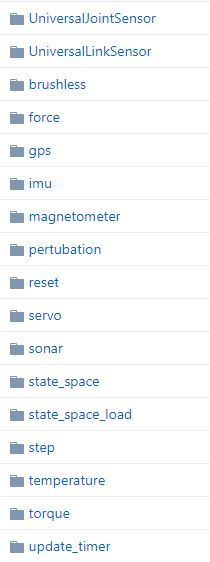
\includegraphics[width=0.45\textwidth]{figuras/plugins.JPG}
\caption{Lista de plugins}
\label{plugins.JPG}
\end{figure}

Mais detalhes leia este tutorial encontrado no site do Gazebo: \url{http://gazebosim.org/tutorials/?tut=plugins\_hello\_world}

\subsection{Plugins Modelo}

\subsubsection{Opções disponibilizadas no ambiente de simulação}

\begin{itemize}
\item Brushless
\begin{itemize}
\item[Descrição:] plugin para simulação das forças de empuxo resultado do giro das duas hélices pelos motores brushless de um tilt-rotor
\item[Arquivo:] libgazebo\_ros\_brushless\_plugin.so
\item[Configurações:]
\begin{itemize}
\item <topic\_FR> </topic\_FR> nome do tópico refente ao valor da força a ser aplicada na hélice direita
\item <topic\_FL> </topic\_FL> nome do tópico refente ao valor da força a ser aplicada na hélice esquerda
\item <topic\_FL> </topic\_FL>
\item <LinkDir> </LinkDir> Elo correspondente à hélice direita (a força será aplicada no eixo z desse elo)
\item <LinkEsq> </LinkEsq> Elo correspondente à hélice esquerda (a força será aplicada no eixo z desse elo)
\end{itemize}
\end{itemize}
\item Servo
\begin{itemize}
\item[Descrição:] plugin para simulação servo motor com funções de Torque e posição
\item[Arquivo:] libgazebo\_servo\_motor\_plugin.so
\item[Configurações]
\begin{itemize}
\item <NameOfJoint> </NameOfJoint> nome da junta a ser controlada pelo servo motor
\item <TopicSubscriber> </TopicSubscriber> nome do tópico com valores de referência para o servo motor
\item <TopicSubscriber> </TopicSubscriber>
\item <LinkDir> </LinkDir> Nome do tópico com valores de sensoriamento do servo (posição e velocidade)
\item <Modo> </Modo> Modo de funcionamento do servo motor
\end{itemize}
\end{itemize}
\item State\_space
\begin{itemize}
\item[Descrição:] plugin para sensoriamento do vetor de estados de um VANT Tilt-rotor. \\ $(x,y,z, \phi,\theta,\psi,\alpha_R,\alpha_L,\frac{dx}{dt},\frac{dy}{dt},\frac{dz}{dt}, \frac{d\phi}{dt},\frac{d\theta}{dt},\frac{d\psi}{dt},\frac{d\alpha_R}{dt},\frac{d\alpha_L}{dt})$
\item[Arquivo:] libgazebo\_AllData\_plugin.so
\item[Configurações]
\begin{itemize}
\item <NameOfTopic> </NameOfTopic> nome do tópico para o usuário obter informações
\item <NameOfJointR> </NameOfJointR> nome a junta do servo motor direito
\item <NameOfJointL> </NameOfJointL> nome a junta do servo motor esquerdo
\item <bodyname> </bodyname> nome do elo correspondente ao corpo principal do servo motor
\end{itemize}
\end{itemize}
\item State\_space\_load
\begin{itemize}
\item[Descrição:] plugin para sensoriamento do vetor de estados de um VANT Tilt-rotor com a função transporte de carga.  \\ $(x,y,z,\phi,\theta,\psi,\alpha_R,\alpha_L,\lambda_x,\lambda_y
\frac{dx}{dt},\frac{dy}{dt},\frac{dz}{dt},\frac{d\phi}{dt},\frac{d\theta}{dt},\frac{d\psi}{dt},\frac{d\alpha_R}{dt},\frac{d\alpha_L}{dt},\frac{d\lambda_x}{dt},\frac{d\lambda_y}{dt})$
\item[Arquivo:] libgazebo\_AllData2\_plugin.so
\item[Configurações]
\begin{itemize}
\item <NameOfTopic> </NameOfTopic> nome do tópico para o usuário obter informações
\item <NameOfJointR> </NameOfJointR> nome a junta do servo motor direito
\item <NameOfJointL> </NameOfJointL> nome a junta do servo motor esquerdo
\item <NameOfJoint\_X> </NameOfJoint\_X> nome a junta correspondente ao grau de liberdade da carga em torno do eixo X
\item <NameOfJoint\_Y> </NameOfJoint\_Y> nome a junta correspondente ao grau de liberdade da carga em torno do eixo Y
\item <bodyname> </bodyname> nome do elo correspondente ao corpo principal do servo motor
\end{itemize}
\end{itemize}
\item temperature
\begin{itemize}
\item[Descrição:] plugin para sensoriamento da temperatura e pressão atmosférica com ruído. \\ 
\item[Arquivo:] libgazebo\_ros\_temperature.so
\item[Configurações]
\begin{itemize}
\item <Topic> </Topic> nome do tópico para o usuário obter dados sensoriais
\item <TempOffset> </TempOffset> offset de erro para dados de temperatura ruidosos
\item <TempStandardDeviation> </TempStandardDeviation> desvio padrão  de erro para dados de temperatura ruidosos
\item <BaroOffset> </BaroOffset> offset de erro para dados de pressão ruidosos
\item <BaroStandardDeviation> </BaroStandardDeviation> desvio padrão  de erro para dados de pressão ruidosos
\item <maxtemp> </maxtemp> valor máximo de temperatura
\item <mintemp> </mintemp> valor mínimo de temperatura
\item <maxbaro> </maxbaro> valor máximo de pressão
\item <minbaro> </minbaro> valor mínimo de pressão
\item <Nbits> </Nbits> quantidade de bits utilizados na digitalização
\end{itemize}
\end{itemize}
\item UniversalJointSensor
\begin{itemize}
\item[Descrição:] plugin para sensoriamento de todos os dados que o Gazebo disponibiliza de uma junta. (ângulo,velocidade angular e Torque)\\ 
\item[Arquivo:] libgazebo\_ros\_universaljoint.so
\item[Configurações]
\begin{itemize}
\item <NameOfTopic> </NameOfTopic> nome do tópico para o usuário obter dados sensoriais
\item <NameOfJoint> </NameOfJoint> nome da junta para sensoriamento
\item <Axis> </Axis> Eixo de rotação da junta (" para primeira junta e "axis2" para segunda junta - gazebo contém juntas q permite dois graus de liberdade)
\end{itemize}
\end{itemize}
\item UniversalLinkSensor
\begin{itemize}
\item[Descrição:] plugin para sensoriamento de todos os dados que o Gazebo disponibiliza de um elo. \\
\item[Ordem de informações]
\begin{itemize}
\item pose relativa em x
\item pose relativa em y
\item pose relativa em z
\item pose relativa em $\phi$
\item pose relativa em $\theta$
\item pose relativa em $\psi$
\item velocidade relativa em x
\item velocidade relativa em y
\item velocidade relativa em z
\item aceleração linear relativa em x
\item aceleração linear relativa em y
\item aceleração linear relativa em z
\item força relativa em x
\item força relativa em y
\item força relativa em z
\item velocidade angular relativa em x
\item velocidade angular relativa em y
\item velocidade angular relativa em z
\item aceleração angular relativa em x
\item aceleração angular relativa em y
\item aceleração angular relativa em z
\item conjugado mecânico relativa em x
\item conjugado mecânico relativa em y
\item conjugado mecânico relativa em z
\item pose global em x
\item pose global em y
\item pose global em z
\item pose global em $\phi$
\item pose global em $\theta$
\item pose global em $\psi$
\item velocidade global em x
\item velocidade global em y
\item velocidade global em z
\item aceleração linear global em x
\item aceleração linear global em y
\item aceleração linear global em z
\item força global em x
\item força global em y
\item força global em z
\item velocidade angular global em x
\item velocidade angular global em y
\item velocidade angular global em z
\item aceleração angular global em x
\item aceleração angular global em y
\item aceleração angular global em z
\item conjugado mecânico global em x
\item conjugado mecânico global em y
\item conjugado mecânico global em z
\item velocidade linear do centro de gravidade global em x
\item velocidade linear do centro de gravidade global em y
\item velocidade linear do centro de gravidade global em z
\item pose linear do centro de gravidade global em x
\item pose linear do centro de gravidade global em y
\item pose linear do centro de gravidade global em z
\end{itemize}

\item[Arquivo:] libgazebo\_ros\_universallink.so
\item[Configurações]
\begin{itemize}
\item <NameOfTopic> </NameOfTopic> nome do tópico para o usuário obter dados sensoriais
\item <NameOfLink> </NameOfLink> nome da elo para sensoriamento
\end{itemize}
\end{itemize}
\end{itemize}

\subsubsection{Inserindo no arquivo de descrição do modelo}

Para inserir plugins modelos basta inserir tags <plugin></plugin>, definindo nome, nome da biblioteca dinâmica e as tags internas necessárias para configuração do plugin. O exemplo abaixo demonstra como referenciar plugins modelo no arquivo SDF. 

\begin{minted}{xml}
<?xml version="1.0" encoding="UTF-8"?>
<sdf version="1.4">
	<model name="modelo">
		<link name="corpo">
			...
		</link>
		<link name="servo">
			...
		</link>
		<joint name="corpo_servo">
			...
		</joint>
		<plugin name="1" filename="1.so">
			<config1> </config1>
			<config2> </config2>
			...
		</plugin>
		<plugin name="2" filename="2.so">
			<config3> </config3>
			<config4> </config4>
			...
		</plugin>
	</model>
</sdf>
\end{minted}

\subsubsection{Processo de criação de novo plugin Modelo}

O processo de criação de um plugin do ponto de vista de desenvolvimento de software consiste na criação de uma classe (composta por arquivos .hpp e .cpp) com interface definida préviamente. No caso, o código fonte deve herdar a interface que está definida na classe ModelPlugin. Esta classe possui três métodos virtuais que são:

\begin{itemize}
\item Init(): método referente ao comportamento personalizado de inicialização do plugin.
\item Load(): Método onde carrega as configurações definidas no arquivo XML, sobretudo ponteiros para acesso a manipulação e sensoriamento de elos e juntas.
\item Reset(): Método para o comportamento personalizado de redefinição do plugin.
\end{itemize}

Mais detalhes na classe pai ModelPlugin podem ser encontrados em \url{http://osrf-distributions.s3.amazonaws.com/gazebo/api/dev/classgazebo_1_1ModelPlugin.html}

A seguir apresenta o exemplo de um código fonte de um plugin model. Neste exemplo é demonstrado a estruturade um arquivo fonte de um plugin e mostrar como os plugins são interrompidos a todo passo de simulação. Detalhes de como programar cada método com o comportamento desejado pode ser utilizado o código fonte deste projeto e o site \url{http://osrf-distributions.s3.amazonaws.com/gazebo/api/}\\

\textbf{Arquivo Exemplo.hpp}

\begin{minted}{c++}
#include <gazebo/physics/physics.hh>
#include <gazebo/transport/TransportTypes.hh>
#include <gazebo/common/Time.hh>
#include <gazebo/common/Plugin.hh>
#include <gazebo/common/Events.hh>
#include <update_timer.h>

namespace gazebo
{
	class Exemplo : public ModelPlugin
	{		
		public: 
		virtual void Init();
		virtual void Load(physics::ModelPtr _model, sdf::ElementPtr _sdf); 
		virtual void Reset();
		
		protected: 
		virtual void Update(); 
		
		private:
		physics::WorldPtr world; 
		UpdateTimer updateTimer;
		event::ConnectionPtr updateConnection;
	};
}
\end{minted}

\textbf{Arquivo Exemplo.cpp}


\begin{minted}{c++}
#include <Exemplo.hpp>

namespace gazebo
{
	void Exemplo::Init()
	{
		// Do something when the plugins starts	
	}
	
	void Exemplo::Load(physics::ModelPtr _model, sdf::ElementPtr _sdf)
	{	
		// Loading data
		world = _model->GetWorld();	
		updateTimer.Load(world, _sdf);
		updateConnection = updateTimer.Connect(boost::bind(&Exemplo::Update, this));
	}
	
	void ServoMotorPlugin::Reset()
	{
		// Do something when reset
	}
	
	void ServoMotorPlugin::Update()
	{
		// Do some something in each simulation time
			
	}
	
	GZ_REGISTER_MODEL_PLUGIN(Exemplo)
}
\end{minted}

Os métodos \textit{Init}, \textit{Load} e \textit{Reset}, como já explicado, realizam, respectivamente comandos de inicilização, leitura de informações do arquivo SDF e reset de simulação. Já o método \textit{Update}, não se encontra na interface do plugin pai \textit{ModelPlugin}, mas é um método que é configurado para ser chamado a todo momento que ocorrer um passo de simulação do Gazebo.

Essa configuração ocorre dentro do método \textit{Load}. Este obtém o ponteiro \textit{\_model} para dados do arquivo SDF do modelo e através do método do conteúdo deste ponteiro \textit{GetWorld}, ele obtém o ponteiro para a estrtura de dados com as informações do cenário. Posteriormente, este estrutura é carregada na classe \textit{UpdateTimer} e é realizado a sua inicialização. Esta estrtura que informa a necessidade de ocorrências de interrupções a cada passos de simulação. 

\subsection{Plugins Mundo}

Um preocupação neste trabalho foi garantir a sincronização entre Controlador (que será descrito posteriormente) e a simulação, conforme ilustrado na figura \ref{flow.jpg}. De forma sequencial os subsistemas serão executados e quando um sistema está executando os outros estão em repouso. Iniciamente, acontece um passo de simulação no Gazebo, os sensores obtém dados do ambiente e manda-os para tópicos de sensores. Em seguida os controladores serão avisados que chegou dados nestes tópicos, assim computará sua lei de controle e enviará os sinais de controle obtidos para tópicos de conexão com atuadores. Por fim os atuadorestrasnmitirão os sinais de controle para o amabiente de simulação.


\begin{figure}[H]
\centering
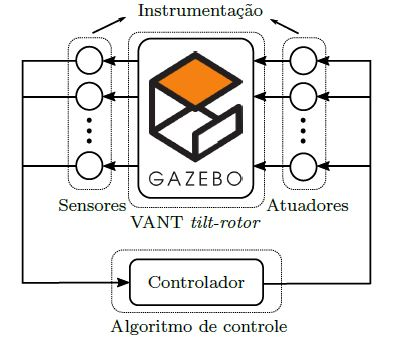
\includegraphics[width=0.65\textwidth]{figuras/flow.jpg}
\caption{Esquemático do simulador}
\label{flow.jpg}
\end{figure}


O controlador é um executável que somente é executado quando chegar novos dados de sensores, no entanto, o Gazebo já é configurado por padrão de rodar indefinidamente. Então com a finalidade de garantir que os componentes do sistem executem sequencialmente, propou-se em deixar o simulador em suspensão e quando necessitar o controlador solicita a execução de novo passo de simulação. Para possibilitar a comunicação do controlador e simulador nesse sentido, projetou-se um plugin mundo que através de uma conxão externa através de tópicos do ROS possibilita que o controlador comande a execução do momento necessário para a execução de novo passo de simulação.

A configuração do plugin mundo é definida como:

\begin{itemize}
\item Step plugin
\begin{itemize}
\item[Descrição:] plugin comando externo do Controlador para solicitação de novo passo de simulação
\item[Arquivo:] libgazebo\_ros\_world\_plugin.so
\item[Configuração:] Nome do tópico definido permanentemente como Step
\end{itemize}
\end{itemize}

\section{Sensores disponíveis}

O sensores, diferentemente dos plugins modelo, são implementados pelo próprio Gazebo e, após serem referenciados no arquivo de descrição do modelo, disponibilizam os seus dados por meio de tópicos do Gazebo. Estes tópicos funcionam semelhantemente aos tópicos do Gazebo, porém possui API própria para lidar com a escrita e leitura de dados. Veja mais detalhes em \url{http://www.robopgmr.com/?p=5614}.

No entanto, como os tópicos do ROS e GAzebo não possuem conexão, é necessário fazer trasnmissão de dados entre ambas as tecnologias de comunicação entre processos. Essa comunicação foi feita, desenvolvendo plugins modelos apenas com essa função. Aqui chamaremos de conversores de dados.

\subsubsection{Opções disponibilizadas}

Diversos são os sensores disponibilizados pelo Gazebo e sua configuração no arquivo SDF estão descritas em \url{http://sdformat.org/spec?ver=1.6&elem=sensor}. Porém apenas alguns coversores de dados foram desenvolvidos para esta versão e são GPS, Sonar, Magnetômetro, IMU. Suas configurações são:

\begin{itemize}
\item GPS
\begin{itemize}
\item[Descrição:] plugin para conversão e transporte de dados entre plugins Gazebo e ROS
\item[Arquivo:] libgazebo\_ros\_sonar.so
\item[Configurações:]
\begin{itemize}
\item <gazebotopic> </gazebotopic> nome do tópico Gazebo
\item <rostopic> </rostopic> nome do tópico ROS
\item <link> </link> nome do elo que o sensor está acoplado
\end{itemize}
\end{itemize}
\end{itemize}

\begin{itemize}
\item Sonar
\begin{itemize}
\item[Descrição:] plugin para conversão e transporte de dados entre plugins Gazebo e ROS
\item[Arquivo:] libgazebo\_ros\_sonar.so
\item[Configurações:]
\begin{itemize}
\item <gazebotopic> </gazebotopic> nome do tópico Gazebo
\item <rostopic> </rostopic> nome do tópico ROS
\item <link> </link> nome do elo que o sensor está acoplado
\end{itemize}
\end{itemize}
\end{itemize}

\begin{itemize}
\item Magnetômetro
\begin{itemize}
\item[Descrição:] plugin para conversão e transporte de dados entre plugins Gazebo e ROS
\item[Arquivo:] libgazebo\_ros\_magnetometer.so
\item[Configurações:]
\begin{itemize}
\item <gazebotopic> </gazebotopic> nome do tópico Gazebo
\item <rostopic> </rostopic> nome do tópico ROS
\item <link> </link> nome do elo que o sensor está acoplado
\end{itemize}
\end{itemize}
\end{itemize}

\begin{itemize}
\item IMU
\begin{itemize}
\item[Descrição:] plugin para conversão e transporte de dados entre plugins Gazebo e ROS
\item[Arquivo:] libgazebo\_ros\_imu.so
\item[Configurações:]
\begin{itemize}
\item <gazebotopic> </gazebotopic> nome do tópico Gazebo
\item <rostopic> </rostopic> nome do tópico ROS
\item <link> </link> nome do elo que o sensor está acoplado
\end{itemize}
\end{itemize}
\end{itemize}

\subsubsection{Inserindo Sensor e conversor no arquivo de descrição de modelo}

Nesta parte será ilustrado como inserir um sensor com seu respectivo conversor de dados no arquivo modelo.




